\documentclass[12pt,a4paper]{styles/report}
\usepackage{mathtext}
\usepackage[utf8x]{inputenc}
\usepackage[T2A]{fontenc}
\usepackage[english, russian]{babel}
\usepackage{textcase}

\usepackage{graphics}
\usepackage{graphicx}
% ����� ��� ����������� ����������� � ���������� � �� ������� \cite � \ref
\usepackage{hyperref}
\usepackage{latexsym}
\usepackage{styles/axodraw}
\usepackage{indentfirst}
\usepackage{cite}
\usepackage{styles/caption-disser}
%\usepackage{flafter}
\usepackage{float}
% ���� ����� ������ ������������ ��� �������� ������ �� ����������
%\usepackage{amsbib}


% ���������� �������� �������� ������ � ���� �������
% !!!!!!!  ����� ������� ������ !!!!!
%\usepackage{showkeys}

% ������ ���������� ��� �������� ����� �������
\frenchspacing

\oddsidemargin=5mm \topmargin=-10mm \headheight=0mm \headsep=0mm
\footskip=10mm \textheight=255mm \textwidth=165mm


\newcommand{\dd}{\mbox{{\rm d}}}
\newcommand{\half}{{\textstyle\frac{1}{2}}}
\newcommand{\third}{{\textstyle\frac{1}{3}}}
\newcommand{\fourth}{{\textstyle\frac{1}{4}}}
\def\lsim{\mathrel{\rlap{\raise 2.5pt \hbox{$<$}}\lower 2.5pt
\hbox{$\sim$}}}
\newcommand{\wmax}{w_{\rm max}}
\renewcommand{\Re}{\mbox{Re}}
\newcommand{\thW}{\theta_{{\rm W}}}
\newcommand{\varepsilonmax}{\varepsilon_{\rm max}}
\newcommand{\Tr}{{\rm Tr}}
\newcommand{\kslash}{\rlap/k}
\newcommand{\qslash}{\rlap/q}
\newcommand{\Order}{{\cal O}}
\newcommand{\TeV}{{\rm TeV}}
\newcommand{\Lumint}{{\cal L}_{\rm int}}


\usepackage[dvips]{color}
\definecolor{Black}{named}{Black}
\definecolor{Red}{named}{Red}
\definecolor{Blue}{named}{Blue}
\newcommand{\black}[1]{\color{Black} #1\color{Black}}
\newcommand{\red}[1]{\color{Red} #1\color{Black}}
\def\change#1{{\red{\sl #1}}}
\def\comment#1{{\small \red{[{\sl #1}]}}}
\newcommand{\blue}[1]{\color{Blue} #1\color{Black}}
\def\change#1{{\blue{\sl #1}}}
\def\comment#1{{\small \blue{[{\sl #1}]}}}

\emergencystretch=30pt

\righthyphenmin=2


%\bibident=0pt

\begin{document}
	
\renewcommand\contentsname{СОДЕРЖАНИЕ}
\renewcommand{\bibname}{СПИСОК ИСПОЛЬЗОВАННЫХ ИСТОЧНИКОВ}
\renewcommand\chaptername{ГЛАВА}
\renewcommand\figurename{Рисунок}
\renewcommand\tablename{Таблица}
\newcommand{\intro}{ВВЕДЕНИЕ}
\newcommand{\prolog}{ПРИЛОЖЕНИЕ}

%%%%%%%%%% Титульный лист
\begin{titlepage}
	\large
	\begin{center}
		\vspace{3mm}
		МИНИСТЕРСТВО ОБРАЗОВАНИЯ РЕСПУБЛИКИ БЕЛАРУСЬ\\
		УЧРЕЖДЕНИЕ ОБРАЗОВАНИЯ\\
		«Гомельский государственный технический университет имени П.О. Сухого»\\
		\vspace{10mm}
		КАФЕДРА «ИНФОРМАЦИОННЫЕ ТЕХНОЛОГИИ»\\
		\vspace{30mm}
		РЕФЕРАТ\\
		на тему\\
			\textbf{\MakeTextUppercase{ Программный комплекс для имитационного моделирования рождения $Z^\prime$ - бозонов в протон-протонных столкновениях с учетом эффектов $Z$ - $Z^\prime$ смешивания
		}}\\
	\vspace{5mm}
		подготовленный для прохождения итоговой аттестации 
		по общеобразовательной дисциплине 
		<<Основы информационных технологи>>\\
	\vspace{40mm}
		Выполнил:\\
		магистрант гр. МАГ 40-12
		специальности 1–40 80 04 <<Математическое моделирование, численные методы и комплексы программ>>\\
		Бурим Илья Павлович
		
	\vspace{15mm}
		Проверил:\\
		доцент кафедры <<Информационные технологии>>\\
		Цитринов А.В.
	\vfill
		Гомель 2017
	\end{center}
\end{titlepage}
%%%%%%%%%%%%%%%

\newpage
\pagestyle{plain} \pagenumbering{arabic} \setcounter{page}{2}
\large \tableofcontents

\newpage
\chapter*{\intro}
\addcontentsline{toc}{chapter}{\intro}
фывфы выфвыф вфывфы

\chapter{BUSINESS INTELLIGENCE AND ANALYTICS: FROM BIG DATA TO BIG IMPACT}
\section{BI\&A 1.0 (Бизнес-анализ и аналитика версия 1.0)}
Firstly the term intelligence has been used by researchers in
artificial intelligence since the 1950s. Business intelligence
became a popular term in the business and IT communities
only in the 1990s. In the late 2000s, business analyticswas
introduced to represent the key analytical component in BI~\cite{Miller:2012a}. More recently big data and big data
analytics have been used to describe the data sets and analytical techniques in applications that are so large (from
terabytes to exabytes) and complex (from sensor to social
media data) that they require advanced and unique data

As a data-centric approach, BI\&A has its roots in the longstanding database management field. It relies heavily on
various data collection, extraction, and analysis technologies~\cite{Chen:2006}. The BI\&A technologies and applications
currently adopted in industry can be considered as BI\&A 1.0,
where data are mostly structured, collected by companies
through various legacy systems, and often stored in commercial relational database management systems (RDBMS). The
analytical techniques commonly used in these systems,
popularized in the 1990s, are grounded mainly in statistical
methods developed in the 1970s and data mining techniques
developed in the 1980s.

Data management and warehousing is considered the foundation of BI\&A 1.0. Design of data marts and tools for
extraction, transformation, and load (ETL) are essential for
converting and integrating enterprise-specific data. Database
query, online analytical processing (OLAP), and reporting
tools based on intuitive, but simple, graphics are used to
explore important data characteristics. Business performance
management (BPM) using scorecards and dashboards help
analyze and visualize a variety of performance metrics. In
addition to these well-established business reporting functions, statistical analysis and data mining techniques are
adopted for association analysis, data segmentation and
clustering, classification and regression analysis, anomaly
detection, and predictive modeling in various business applications. Most of these data processing and analytical technologies have already been incorporated into the leading commercial BI platforms offered by major IT vendors including
Microsoft, IBM, Oracle, and SAP~\cite{Salton:1989}.

Among the 13 capabilities considered essential for BI platforms, according to the Gartner report by Sallam et al. (2011),
the following eight are considered BI\&A 1.0: reporting,
dashboards, ad hocquery, search-based BI, OLAP, interactive
visualization, scorecards, predictive modeling, and data
mining. A few BI\&A 1.0 areas are still under active development based on the Gartner BI Hype Cycle analysis for
emerging BI technologies, which include data mining workbenchs, column-based DBMS, in-memory DBMS, and realtime decision tools (Bitterer 2011). Academic curricula in
Information Systems (IS) and Computer Science (CS) often include well-structured courses such as database management
systems, data mining, and multivariate statistics.

In conclusion the opportunities associated with data and analysis in different organizations have helped generate significant interest
in BI\&A, which is often referred to as the techniques, technologies, systems, practices, methodologies, and applications
that analyze critical business data to help an enterprise better
understand its business and market and make timely business
decisions. 
\section{BI\&A 2.0}
This chapter presents the Internet and the Web. These technologies began to offer
unique data collection and analytical research and development opportunities. In 2000s the HTTP-based Web 1.0 systems,
characterized by Web search engines such as Google and
Yahoo and e-commerce businesses such as Amazon and
eBay, allow organizations to present their businesses online
and interact with their customers directly. 
In addition to porting their traditional RDBMS-based product information
and business contents online, detailed and IP-specific user
search and interaction logs that are collected seamlessly
through cookies and server logs have become a new gold
mine for understanding customers’ needs and identifying new
business opportunities. Web intelligence, web analytics, and
the user-generated content collected through Web 2.0-based
social and crowd-sourcing systems (Doan et al. 2011;
O’Reilly 2005) have ushered in a new and exciting era of
BI\&A 2.0 research in the 2000s, centered on text and web
analytics for unstructured web contents.

An immense amount of company, industry, product, and
customer information can be gathered from the web and
organized and visualized through various text and web mining
techniques. By analyzing customer clickstream data logs,
web analytics tools such as Google Analytics can provide a
trail of the user’s online activities and reveal the user’s
browsing and purchasing patterns. Web site design, product
placement optimization, customer transaction analysis, market
structure analysis, and product recommendations can be
accomplished through web analytics. The many Web 2.0
applications developed after 2004 have also created an abundance of user-generated content from various online social
media such as forums, online groups, web blogs, social networking sites, social multimedia sites (for photos and videos),
and even virtual worlds and social games (O’Reilly 2005). In
addition to capturing celebrity chatter, references to everyday
events, and socio-political sentiments expressed in these
media, Web 2.0 applications can efficiently gather a large
volume of timely feedback and opinions from a diverse
customer population for different types of businesses.

Many marketing researchers believe that social media
analytics presents a unique opportunity for businesses to treat
the market as a “conversation” between businesses and
customers instead of the traditional business-to-customer,
one-way “marketing” (Lusch et al. 2010). Unlike BI\&A 1.0
technologies that are already integrated into commercial
enterprise IT systems, future BI\&A 2.0 systems will require
the integration of mature and scalable techniques in text
mining (e.g., information extraction, topic identification,
opinion mining, question-answering), web mining, social
network analysis, and spatial-temporal analysis with existing
DBMS-based BI\&A 1.0 systems.

Except for basic query and search capabilities, no advanced
text analytics for unstructured content are currently considered in the 13 capabilities of the Gartner BI platforms.
Several, however, are listed in the Gartner BI Hype Cycle,
including information semantic services, natural language
question answering, and content/text analytics (Bitterer 2011). 
New IS and CS courses in text mining and web mining have
emerged to address needed technical training.

In conclusion it can be notified that in 2000s, BI\&A created big jump in infrastructure natural language, information extraction, topic identification, opinion mining, question-answering. And created new directions in IT.

\section{BI\&A 3.0 (Бизнес-анализ и аналитика версия 3.0)}
This chapter describes most of the academic research on mobile BI, opening up exciting new steams of innovative applications and describes business intelligence and analytics in Web 3.0 area.

Whereas web-based BI\&A 2.0 has attracted active research
from academia and industry, a new research opportunity in
BI\&A 3.0 is emerging. As reported prominently in an
October 2011 article in The Economist (2011), the number of
mobile phones and tablets (about 480 million units) surpassed
the number of laptops and PCs (about 380 million units) for
the first time in 2011. Although the number of PCs in use
surpassed 1 billion in 2008, the same article projected that the
number of mobile connected devices would reach 10 billion
in 2020. Mobile devices such as the iPad, iPhone, and other
smart phones and their complete ecosystems of downloadable
applicationss, from travel advisories to multi-player games,
are transforming different facets of society, from education to
healthcare and from entertainment to governments. Other
sensor-based Internet-enabled devices equipped with RFID,
barcodes, and radio tags (the “Internet of Things”) are
opening up exciting new steams of innovative applications.
The ability of such mobile and Internet-enabled devices to
support highly mobile, location-aware, person-centered, and
context-relevant operations and transactions will continue to
offer unique research challenges and opportunities throughout
the 2010s. Mobile interface, visualization, and HCI
(human–computer interaction) design are also promising
research areas. Although the coming of the Web 3.0 (mobile
and sensor-based) era seems certain, the underlying mobile
analytics and location and context-aware techniques for
collecting, processing, analyzing and visualizing such largescale
and fluid mobile and sensor data are still unknown.

No integrated, commercial BI\&A 3.0 systems are foreseen for
the near future. Most of the academic research on mobile BI
is still in an embryonic stage. Although not included in the
current BI platform core capabilities, mobile BI has been
included in the Gartner BI Hype Cycle analysis as one of the
new technologies that has the potential to disrupt the BI
market significantly~\cite{Blei:2012}. The uncertainty associated
with BI\&A 3.0 presents another unique research
direction for the IS community.
Table 1 summarizes the key characteristics of BI\&A 1.0, 2.0,
and 3.0 in relation to the Gartner BI platforms core capabilities
and hype cycle.

In conclusion it can be notified that the decade of the 2010s was an exciting one for high-impact BI\&A research and development for both industry and academia. IS research and education programs
need to carefully evaluate future directions, curricula,
and action plans, from BI\&A 1.0 to 3.0. The business community and industry have already taken important steps to adopt BI\&A for their needs. The IS community faces unique challenges and opportunities
in making scientific and societal impacts that are relevant and
long-lasting~\cite{Chen:2006}. 
\section{BI\&A Applications: From Big Data to Big Impact (Бизнес-анализ и аналитика приложений: от больших данных к большому результату)}

This chapter describes new streams where business intelligence and analytics big data will be used. Streams like international travel, high-speed network connections, global supply-chain, and
outsourcing have created a tremendous opportunity for IT
advancement. It predicted by Thomas Freeman in his seminal
book, The World is Flat (2005).

Several global business and IT trends have helped shape past
and present BI\&A research directions. In addition to ultra-fast
global IT connections, the development and deployment of
business-related data standards, electronic data interchange
(EDI) formats, and business databases and information
systems have greatly facilitated business data creation and
utilization. The development of the Internet in the 1970s and
the subsequent large-scale adoption of the World Wide Web
since the 1990s have increased business data generation and
collection speeds exponentially. Recently, the Big Data era
has quietly descended on many communities, from governments
and e-commerce to health organizations. With an
overwhelming amount of web-based, mobile, and sensorgenerated
data arriving at a terabyte and even exabyte scale~\cite{Gelfand:2012}, new science, discovery, and
insights can be obtained from the highly detailed, contextualized,
and rich contents of relevance to any business or
organization.

In addition to being data driven, BI\&A is highly applied and
can leverage opportunities presented by the abundant data and
domain-specific analytics needed in many critical and highimpact
application areas. Several of these promising and
high-impact BI\&A applications are presented below, with a
discussion of the data and analytics characteristics, potential
impacts, and selected illustrative examples or studies: (1) ecommerce
and market intelligence, (2) e-government and
politics 2.0, (3) science and technology, (4) smart health and
well-being, and (5) security and public safety. By carefully
analyzing the application and data characteristics, researchers
and practitioners can then adopt or develop the appropriate
analytical techniques to derive the intended impact. IS departments thus face unique opportunities and
challenges in developing integrated BI\&A research and
education programs for the new generation of data/analyticssavvy
and business-relevant students and professionals~\cite{Chen:2011b}.

In conclusion to technical system implementation, significant business
or domain knowledge as well as effective communication
skills are needed for the successful completion of such BI\&A
projects.
\section{E-Commerce and Market Intelligence}

The excitement surrounding BI\&A and Big Data has arguably
been generated primarily from the web and e-commerce
communities. Significant market transformation has been
accomplished by leading e-commerce vendors such Amazon
and eBay through their innovative and highly scalable ecommerce
platforms and product recommender systems.
Major Internet firms such as Google, Amazon, and Facebook
continue to lead the development of web analytics, cloud
computing, and social media platforms. The emergence of
customer-generated Web 2.0 content on various forums,
newsgroups, social media platforms, and crowd-sourcing
systems offers another opportunity for researchers and practitioners to “listen” to the voice of the market from a vast
number of business constituents that includes customers, employees,
investors, and the media (Doan et al. 2011; O’Rielly
2005). Unlike traditional transaction records collected from
various legacy systems of the 1980s, the data that e-commerce
systems collect from the web are less structured and often
contain rich customer opinion and behavioral information.
For social media analytics of customer opinions, text analysis
and sentiment analysis techniques are frequently adopted
(Pang and Lee 2008). Various analytical techniques have also
been developed for product recommender systems, such as
association rule mining, database segmentation and clustering,
anomaly detection, and graph mining (Adomavicius and
Tuzhilin 2005). Long-tail marketing accomplished by
reaching the millions of niche markets at the shallow end of
the product bitstream has become possible via highly targeted
searches and personalized recommendations (Anderson
2004).
The Netfix Prize competition2
for the best collaborative
filtering algorithm to predict user movie ratings helped generate
significant academic and industry interest in recommender
systems development and resulted in awarding the grand prize
of \$1 million to the Bellkor’s Pragmatic Chaos team, which
surpassed Netflix’s own algorithm for predicting ratings by
10.06 percent. However, the publicity associated with the
competition also raised major unintended customer privacy
concerns.

Much BI\&A-related e-commerce research and development
information is appearing in academic IS and CS papers as
well as in popular IT magazines.
\section{E-Government and Politics 2.0}

This chapter describes cahnges e-commerce area with coming Web 2.0
and with coming new technologies in BI\&A research. The advent of Web 2.0 has generated much excitement for
reinventing governments. 

The 2008 U.S. House, Senate, and
presidential elections provided the first signs of success for
online campaigning and political participation. Dubbed
<<politics 2.0>>, politicians use the highly participatory and
multimedia web platforms for successful policy discussions,
campaign advertising, voter mobilization, event announcements,
and online donations. As government and political
processes become more transparent, participatory, online, and
multimedia-rich, there is a great opportunity for adopting
BI\&A research in e-government and politics 2.0 applications.
Selected opinion mining, social network analysis, and social
media analytics techniques can be used to support online
political participation, e-democracy, political blogs and
forums analysis, e-government service delivery, and process
transparency and accountability (Chen 2009; Chen et al.
2007). For e-government applications, semantic information
directory and ontological development (as exemplified below)
can also be developed to better serve their target citizens.

Despite the significant transformational potential for BI\&A in
e-government research, there has been less academic research
than, for example, e-commerce-related BI\&A research. Egovernment
research often involves researchers from political
science and public policy. For example, Karpf (2009) analyzed
the growth of the political blogosphere in the United
States and found significant innovation of existing political
institutions in adopting blogging platforms into their Web
offerings. In his research, 2D blogspace mapping with composite
rankings helped reveal the partisan makeup of the
American political blogsphere. Yang and Callan (2009)
demonstrated the value for ontology development for government
services through their development of the OntoCop
system, which works interactively with a user to organize and
summarize online public comments from citizens.

In conclusion it can be notified that e-commerce area will be grow with BI\&A science. Also it can be notified that more important for e-commerce will be the BI\&A in e-government research and e-commerce-related BI\&A research directions.
\section{Science and Technology}

This chapter describes using business intelligence and analytics big data for science. Describes tools and algorithms for successful opening of new achievements and researchs.

Many areas of science and technology (S\&T) are reaping the
benefits of high-throughput sensors and instruments, from
astrophysics and oceanography, to genomics and environmental
research. To facilitate information sharing and data
analytics, the National Science Foundation (NSF) recently
mandated that every project is required to provide a data
management plan. Cyber-infrastructure, in particular, has
become critical for supporting such data-sharing initiatives.

The 2012 NSF BIGDATA program solicitation is an obvious
example of the U.S. government funding agency’s concerted
efforts to promote big data analytics. The program
aims to advance the core scientific and technological
means of managing, analyzing, visualizing, and extracting
useful information from large, diverse, distributed
and heterogeneous data sets so as to accelerate
the progress of scientific discovery and innovation;
lead to new fields of inquiry that would not
otherwise be possible; encourage the development of
new data analytic tools and algorithms; facilitate
scalable, accessible, and sustainable data infrastructure;
increase understanding of human and social
processes and interactions; and promote economic
growth and improved health and quality of life.

Several S\&T disciplines have already begun their journey
toward big data analytics. For example, in biology, the NSF
funded iPlant Collaborative is using cyberinfrastructure to
support a community of researchers, educators, and students
working in plant sciences. iPlant is intended to foster a new
generation of biologists equipped to harness rapidly expanding
computational techniques and growing data sets to
address the grand challenges of plant biology. The iPlant data
set is diverse and includes canonical or reference data,
experimental data, simulation and model data, observational
data, and other derived data. It also offers various open
source data processing and analytics tools.

In astronomy, the Sloan Digital Sky Survey (SDSS) shows
how computational methods and big data can support and
facilitate sense making and decision making at both the
macroscopic and the microscopic level in a rapidly growing
and globalized research field. The SDSS is one of the most
ambitious and influential surveys in the history of astronomy.
Over its eight years of operation, it has obtained deep, multicolor
images covering more than a quarter of the sky and
created three-dimensional maps containing more than 930,000
galaxies and over 120,000 quasars. Continuing to gather data
at a rate of 200 gigabytes per night, SDSS has amassed more
than 140 terabytes of data. The international Large Hadron
Collider (LHC) effort for high-energy physics is another
example of big data, producing about 13 petabytes of data in
a year (Brumfiel 2011).

In conclusion it can be notified that business intelligence and analytics big data contributed to the big jump in astronomy, physics  high-energy. The relationship between BI\&A and science contributed to delevopment of new data processing and analytics tools, algorithms.

%\chapter{Рождения $Z^\prime$ - бозонов в протон-протонных столкновениях с учетом эффектов $Z$ - $Z^\prime$ смешивания}
%\section{Новая физика}

Несмотря на впечатляющий успех в описании экспериментов, Стандартная модель не может считаться окончательной теорией элементарных частиц. У нее есть свои трудности. Физики уверены, что она должна быть частью некоторой более глубокой теории строения микромира, той частью, которая видна в экспериментах на коллайдерах при энергиях ниже примерно 1 ТэВ. Главная задача Большого адронного коллайдера — получить хотя бы первые намеки на то, что это за более глубокая теория.

Теоретики разработали большое число кандидатов на такую теорию. Все они, естественно, включают какие-то элементы, которые отсутствуют в Стандартной модели. Часто такие теории коллективно называют «Новая физика» или «За пределами Стандартной модели». На этой странице перечислены некоторые из активно изучаемых вариантов Новой физики~\cite{2part-1}.

Суперсимметрия — это гипотетическая симметрия между фермионами и бозонами. Теории, использующие эту идею, оказываются удивительно мощными, и потому именно с суперсимметрией многие связывают надежды на открытие физики за пределами Стандартной модели. Однако до сих пор не было получено ни одного убедительного доказательства в пользу того, что суперсимметрия реализуется в нашем мире. Ее поиск является одной из главных задач Большого адронного коллайдера.
\begin{figure}[h]
	\centering
	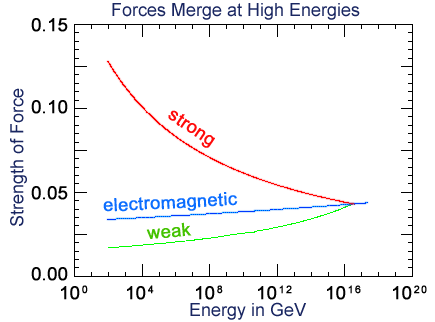
\includegraphics[width=\textwidth]{figures/hep-sm.png}
	\caption{Константы связи трех типов взаимодействий}
	\label{fig:fig01}
\end{figure}
Константы связи трех взаимодействий частиц в микромире сходятся к одному значению, если имеющиеся сейчас данные экстраполировать в область очень высоких энергий. Это совпадение считается неслучайным и воспринимается физиками как намек на то, что все три взаимодействия при больших энергиях объединяются в одно.

В XIX веке физики обнаружили, что электричество и магнетизм — это две стороны одной медали, электромагнитного взаимодействия. Век спустя, при создании Стандартной модели, электромагнетизм и слабые ядерные силы были объединены в рамках единого электрослабого взаимодействия. (Точнее говоря, внутри электрослабого взаимодействия имеются по-прежнему две разные силы, а электромагнитное и слабое взаимодействия возникают как комбинации этих сил). Каждое такое объединение упрощало теорию, уменьшало количество введенных в нее «сущностей», переводило наше понимание микромира на новый уровень.

Сейчас физики имеют сразу несколько причин подозревать, что при очень высоких энергиях происходит объединение электрослабого и сильного взаимодействий (рисунок 2.1). Модели, использующие эту идею (так называемые Теории великого объединения) разрабатываются уже давно. В идеале хотелось бы, чтобы такая теория естественным образом объясняла, почему фундаментальных взаимодействий именно столько и именно с такими свойствами, а также имела четкие предсказания, доступные проверке в современных экспериментах.

При энергиях элементарных частиц, доступных на ускорителях, гравитация по-прежнему остается исключительно слабой, так что заметить ее проявления не удается. Однако ее сила растет с ростом энергии, и при энергиях столкновения порядка планковской она станет столь же важной, как и другие взаимодействия. В этом случае в полный рост встает исключительно сложный вопрос о том, как включить гравитацию в квантовое описание микромира. Поскольку гравитация в современной физике считается проявлением кривизны пространства-времени, успешная теория с сильной гравитацией должна описывать в рамках единого формализма не только все взаимодействия и всё вещество, но и структуру пространства-времени.

Одним из наиболее привлекательных путей решения этого вопроса является теория суперструн и ее дальнейшее развитие в виде теории бран и М-теории. В этих теориях считается, что фундаментальными объектами, существующими в многомерной вселенной, являются не точечные частицы, а протяженные объекты -- струны, мембраны и еще более многомерные образования. В этой теории были получены впечатляющие успехи при высоких энергиях, однако при попытке вывести свойства нашего низкоэнергетического мира из теории суперструн возникает обескураживающая неопределенность предсказаний.

Долгое время казалось, что проверка предсказаний теории суперструн лежит далеко за пределами возможностей человечества, поскольку речь идет об энергиях, на 15 порядков превышающих энергии современных ускорителей. Однако примерно 10 лет назад возникло новое направление развития теории, в котором гравитация становится сильной на энергиях порядка 1 ТэВ. Такая возможность возникает в том случае, если наш мир более чем трехмерный и если при этом новые дополнительные пространственные размерности достаточно протяженны: либо они бесконечны, либо свернуты в многомерные петельки размером много больше ядерного масштаба.

В этом случае на \textit{LHC} следует ожидать целый ряд совершенно замечательных эффектов, отсутствующих в Стандартной модели, например, рождение гравитонов, которые будут улетать из нашего мира в дополнительные измерения, и микроскопических черных дыр, тут же испаряющихся с испусканием множества обычных частиц. Будут также наблюдаться сильные отклонения от предсказаний Стандартной модели в столкновении обычных частиц. Стоит, впрочем, подчеркнуть, что пока нет никаких экспериментальных подтверждений того, что эта красивая гипотеза имеет отношение к нашему миру.

Все три перечисленные выше направления «Новой физики» опираются на глубокие теоретические гипотезы об устройстве нашего мира (суперсимметрия, единство сил, квантово-гравитационная вселенная). Однако кроме этих направлений теоретики также рассматривают разнообразные теории «статусом пониже». В этих теориях просто отмечается, что текущие экспериментальные данные не запрещают те или иные экзотические объекты или явления, и разрабатываются их следствия. Вот несколько примеров таких моделей разной степени экзотичности.

\begin{figure}[h]
	\centering
	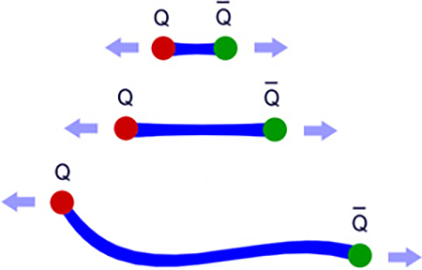
\includegraphics[width=\textwidth]{figures/quirk-antiquirk.jpg}
	\caption{Кварки}
	\label{fig:fig03}
\end{figure}

Неминимальные хиггсовские модели. Поскольку хиггсовские бозоны — единственные частицы Стандартной модели, до сих пор не открытые экспериментально, теоретики изучают самые разные варианты устройства этого сектора теории.
Новые поколения фермионов. Можно предположить, что кроме трех известных поколений кварков и лептонов существуют и другие поколения. Частицы из этих поколений должны быть очень тяжелыми, иначе бы их уже давно открыли в эксперименте.

Новые короткодействующие силы. В таких моделях предполагается, что в нашем мире есть и иные силовые взаимодействия, отличные от сильных, слабых и электромагнитных, но они настолько короткодействующие, что до сих пор никак не проявлялись в эксперименте. На Большом адронном коллайдере благодаря его рекордной энергии удается «прощупать» взаимодействия частиц на исключительно малых расстояниях (менее 10–19 метра), а значит, появляется шанс эти взаимодействия обнаружить. Они могут проявляться либо как рождение и распад частицы-переносчика новых сил (такие гипотетические частицы обозначают $Z^\prime$), либо как усиленное рассеяние частиц на большие углы.

Лептокварки. В Стандартной модели и в подавляющем большинстве теорий Новой физики кварки и лептоны взаимодействуют друг с другом опосредованно, путем обмена квантами силовых полей. Однако можно представить себе возможность того, что кварки и лептоны исходно являлись фермионами одного типа и лишь потом расщепились на два разных сорта. В таком случае должны существовать новые тяжелые частицы — лептокварки, которые распадаются прямо на кварк и лептон. Подобные частицы встречаются в теориях Великого объединения.

Квирки. Одним из очень необычных и любопытных вариантов новых сил является гипотеза квирков (\textit{quirks}). Эта модель построена по типу обычного сильного взаимодействия: в ней предполагается, что существует новое силовое поле с конфайнментом и новые частицы, его чувствующие. Если частицы очень тяжелые, то между ними будут натягиваться длинные, даже макроскопические силовые струны, которые не смогут порваться (рисунок 2.2).

Слабое взаимодействие – короткодействующее фундаментальное взаимодействие между элементарными частицами, ответственное за бета-распад атомных ядер и медленные распады частиц. Слабое взаимодействие значительно слабее сильного и электромагнитного, но гораздо сильнее гравитационного. В слабом взаимодействии участвуют все фундаментальные фермионы (кварки и лептоны) и все адроны. Единственными частицами, которые участвуют только в слабом взаимодействии являются три типа нейтрино $v_e$, $v_\mu$, $v_\tau$ и их античастицы  антинейтрино $\bar{v_e}$,  антинейтрино $\bar{v_\mu}$,  антинейтрино $\bar{v_\tau}$. В нем не участвуют переносчики сильного, электромагнитного и гравитационного взаимодействий -- глюон, фотон и гравитон. В процессе слабого взаимодействия частицы обмениваются переносчиками слабого взаимодействия промежуточными (фундаментальными) бозонами: имеющими электрический заряд $W^±$ и нейтральным $Z$. Эти бозоны, в отличие от переносчиков остальных фундаментальных сил безмассовых глюона, фотона и гравитона, имеют огромные массы $m_W$ = 80.4 ГэВ/с~${}^2$ и $m_Z$ = 91.2 ГэВ/с${}^2$ (примерно как у атомов циркония или ниобия), что приводит к очень малому радиусу действия слабых сил ≈10-18 см (что на три порядка меньше радиуса сильного взаимодействия) и очень низкой по сравнению с сильными и электромагнитными процессами вероятности (скорости) слабых процессов.

Несмотря на малую величину и короткодействие слабые силы играют очень важную роль в природе. Так без них погасло бы Солнце, так как внутри него остановился бы процесс превращения 4 протонов в ядро гелия-4, являющийся основным источником энергии Солнца.

Слабое взаимодействие выделяется тем, что в нём не соблюдается ряд запретов, присущих сильному и электромагнитному взаимодействиям. Так в слабых процессах кварки одного типа (аромата) превращаются в кварки других ароматов~\cite{nuclphys:weak}.

Особенности слабого взаимодействия

\begin{itemize}
	\item[--] Их слабость (медленноеть), выражающаяся в том, что
	вероятность этих процессов на много порядков меньше
	вероятностей сильных и электромагнитных процессов.
	
	\item[--] Малый радиус взаимодействия —как минимум на
	два порядка меньший, чем радиус сильного взаимодействия.
	Ни в одном из слабых процессов не удалось до 1982 г. обнаружить каких-либо отклонений от точечного четырех-
	фермионного взаимодействия.
	
	\item[--] Сильное, максимально возможное несохранение пространственной и зарядовой четностей. Так, в заряженные
	токи входят только левые компоненты спиноров, описывающих частицы, и только правые компоненты спиноров,
	описывающих античастицы.
	
	\item[--] Несохранение \textit{СР}-четности.
	
	\item[--] Несохранение ароматов (странности, чарма и т. д.).
	
	\item[--]  То обстоятельство, что только в слабых взаимодействиях принимают участие нейтрино.
	
\end{itemize}

Тем поразительней, что, несмотря на столь резкие отличия, слабые и электромагнитные взаимодействия представляют собой, по-видимому, проявление одного и того же
взаимодействия, которое в последние годы получило название электрослабого.

Согласно электрослабой теории слабые взаимодействия
заряженных токов обусловлены обменами $W$-бозонами, а
нейтральных -- $Z$-бозонами, подобно тому как взаимодействие электромагнитных токов обусловлено обменом фотонами. При этом слабость и малый радиус слабого взаимодействия объясняются тем, что, в отличие от фотонов, $W$ и $Z$-бозоны -- очень тяжелые частицы Остальные особенности слабого взаимодействия прямо заложены в предположении о форме исходных фермионных токов теории.
Так что в злектрослабой теории удивляться надо не тому,
что слабое взаимодействие зеркально-асимметрично, a то-
му, что электромагнитное -- зеркально-симмеnгричное.

Слабое взаимодействие переносится массивными $W^±$- и $Z$-бозонами. Обмен заряженными $W^+$ и $W^-$-бозонами приводит к изменению электрического заряда взаимодействующих фермионов. Эти процессы происходят за счет заряженных токов.




%\section{Инструменты имитационного моделирования}



Для исследования отклика детектора на различные физические процессы, созданы программы, позволяющие перевести моделированное на уровне частиц событие  взаимодействия протонов при соударении в формат представления данных детекторов установки \textit{ATLAS}. Алгоритмы моделирования интегрированы в программную оболочку эксперимента  \textit{ATLAS}, именуемую \textit{Athena}, использующую программный пакет \textit{GEANT4}.

Генератор события создает набор частиц, который направляется в программу быстрого или полного моделирования детектора. Генераторы событий встроены в \textit{Athena}. Используется большое число других, поддерживаемых авторами, генераторов, которые имеют блоки связи для использования в \textit{Athena}. Основной массив модельных событий создан с помощью генераторов \textit{PYTHIA}~\cite{2part-pythia-all}, включая его версию \textit{PYTHIAВ},  предназначенную в  \textit{ATLAS} для моделирования событий с рождением \textit{В}-адронов.

\textit{PYTHIA} - это программного пакета для визуализации результатов моделирования процессов столкновения частиц при высоких энергиях осуществляющего генерацию методом Монте-Карло физических событий.

Программы \textit{PYTHIA} интенсивно используются для генерации событий в физике высоких энергий при описании процессов множественного рождения в столкновениях элементарных частиц. В частности задачи, что включает решаемые жесткие с взаимодействия помощью данного в столкновениях $e^+e^-$, $pp$ и $ep$, а также некоторые другие случаи. Программа предназначенна для генерации генератора полных событий, т.е. дают более детальную картину, чем мы наблюдаем в эксперименте, в рамках нашего понимания фундаментальной физики процессов. Обсуждаемые здесь программы Монте-Карло построены как ведомые системы, т.е. пользователь должен написать основную программу. Из нее различные программы вызываются для выполнения частных задач, после чего управление снова передается основной программе. Некоторые из этих задач могут быть весьма тривиальными, и достаточно высокоуровневые программы могут производить большое число вызовов подпрограмм.

Генераторы общего назначения создают событие как целое. Они используют много параметров, часть из которых относится к фундаментальным параметрам, такие как константы связи квантовой хромодинамики (КХД) и электрослабой теории, часть относится к моделям, описывающим взаимодействия на больших расстояниях, с малыми передачами импульса, т.н. «мягкой» КХД, и к электрослабым процессам.

Для корректного моделирования процессов рождения и распада частиц необходимо учитывать условия проведения эксперимента. Это условия рождения изучаемых частиц на ускорителе при соответствующих энергиях сталкивающихся пучков, полные цепочки распадов частиц до уровня <<стабильных частиц>>, регистрируемых детектором. Для решения этих задач применяются генераторы событий, использующие метод Монте-Карло.
Генератор \textit{PYTHIA} является широко используемой в физике высоких энергий программой моделирования столкновений различных частиц в широком диапазоне энергий. Этот генератор учитывает процессы фрагментации кварков в адроны и разыгрывает сложные цепочки адронных распадов. Стартуя с заданного пользователем процесса, (столкновение двух протонов с рождением \textit{Z}-бозона и т.п.) программа случайным образом (с учетом законов сохранения и, по возможности, теоретически известной структуры взаимодействия) разыгрывает конфигурацию конечных партонов, а затем моделирует т.н. процесс адронизации - процесс превращения ненаблюдаемых кварков и глюонов в реальные стабильные и нестабильные частицы с последующим распадом нестабильных частиц. На выходе программа выдает список всех частиц, родившихся в результате столкновения заданных первичных частиц, значения их компонент импульса и энергии. Кроме того, имеется возможность проследить последовательность рождений и распадов от первичного взаимодействия до рождения данной частицы. В качестве входных параметров программы используются описания сталкивающихся частиц, их энергий и тип моделируемого процесса (например, рождение \textit{Z}-бозона). Существующие версии пакета \textit{РYTHIА} написаны на языке программирования \textit{FORTRAN}.
Результаты генерации -- характеристики вторичных частиц -- записываются в файл, что позволяет в дальнейшем проводить статистическую обработку событий.
%\section{Распады промежуточных бозонов. Определение массы $Z^\prime$-бозона}

В физических программаx экспериментов на  современных  дронных (\textit{LHC}) и планируемых на  электрон-позитронных (\textit{ILC, CLIC}) коллайдерах вопросу поиск  <<новой>> физики, выходящей за  рамки Стандартной модели (СМ), традиционно уделяется большое внимание. К числу подобных теоретических построений, являющихся обобщением СМ, относятся модели с расширенным к либровочным сектором, такие как лево-правосиммет- 
ричные модели (\textit{LR}), альтернативные лево-правосимметричные модели (\textit{ALR}), $E_6$-модели
и др.~\cite{Bobovnikov:2016}. Их исследование (теоретическое и экспериментальное) представляет значи-тельный интерес. Эти модели являются одними из простейших расширений СМ, характеризующихся элементарной структурой хиггсовского сектора. Общим для данных моделей является то, что они предсказывают новые физические объекты и явления на масштабе энергий $O$ (1 ТэВ), связанные, например, с наличием тяжелых нейтральных ($Z^\prime$) калибровочных бозонов, обусловленных дополнительными калибровочными симме-триями $U(1)^\prime$.

Достижение порога рождения $Z^\prime$-бозона явилось бы прямым доказательством про-явления «новой» физики. Однако в данном случае интервал поиска масс $Z^\prime$ ограничен максимальной энергией коллайдера, на котором проводятся эксперименты. Значительно более широкий интервал масс можно исследовать с помощью пропагаторных эффектов. В этом случае ведется поиск отклонений различных наблюдаемых от соответствующих предсказаний СМ. Если экспериментальные данные при достигнутом уровне точности согласуются с СМ, т. е. отклонений от предсказаний СМ нет, то эту экспериментальную информацию можно использовать для получения ограничений на динамические параметры и массы $Z^\prime$-бозонов.

Потенциальные возможности $e^+$$e^-$-коллайдеров для прямого рождения новых калибровочных бозонов гораздо скромнее по сравнению с адронными машинами из-за более низких энергий пучков. Кроме того, современные ограничения на массы $Z^\prime$-бозонов для большинства моделей превосходят планируемую энергию электрон-позитронного коллайдера \textit{ILC}, $\sqrt{s}<< M_{Z^\prime}$. Тем не менее основным достоинством этих машин является возможность проведения экспериментов по измерению наблюдаемых величин с высокой степенью точности и получения однозначной информации о косвенных (виртуальных) эффектах новых $Z^\prime$-бозонов, а также эффектах бозонного $Z$-$Z^\prime$-смешивания. Последние, в моделях с расширенным калибровочным сектором, зависят от структуры хиггсовского сектора модели. Тем самым экспериментальное исследование процессов рождения пар $W^±$-бозонов может не только пролить свет на возможное существование <<новой>> физики, но и дать косвенные указания на хиггсовскую природу, а также установить структуру модели.

На основе данных, полученных из низкоэнергетических экспериментов по нейтральным токам, результатов на $e^+e^-$-коллайдерах \textit{LEP} и \textit{SLC}~\cite{Bobovnikov:2016}, а также недавно выполненных экспериментов по поиску прямого адронного рождения $Z^\prime$-бозонов в процессе Дрелла-Яна.
\begin{center}
	$pp \rightarrow Z^\prime \rightarrow l^+l^- + X$
\end{center}
($l=e,\mu$) на коллайдере \textit{LНC} при энергии $\sqrt{s}$ = 7 и 8 ТэВ с интегральной светимостью соответственно $L_int$ = 5 и 20 фб${}^{-1}$~\cite{Bobovnikov:2016} можно заключить, что для большинства расширенных калибровочных моделей граничные значения для масс дополнительных $Z^\prime$- бозонов находятся в интервале $\sim$ 2,5-3,0 ТэВ (в зависимости от модели), а современный масштаб ограничений на угол смешивания составляет $\mathcal{O}(\varphi )$ ~ ${10}^{-2}$--${10}^{-3}$ рад. При этом наиболее точная информация об угле смешивания была получена преимуще¬ственно из экспериментов на электрон-позитронных коллайдерах \textit{LEP1}~\cite{schael:2006} и \textit{SLC} по измерению резонансных наблюдаемых физических величин при энергии начальных состояний, равной массе стандартного $Z$-бозона, $\sqrt{s}$ = $M_Z$, в процессах
\begin{center}
	$e^+e^- \rightarrow f\bar{f}$
\end{center}

где конечными фермионными состояниями $f$ были заряженные лептоны и кварки~\cite{andreev-pankov:2012}. Высокая точность, достигнутая в экспериментах на коллайдерах \textit{LEP1} и \textit{SLC}, объясняется прежде всего возможностью набора большого объема данных в резонансной области энергии.

Кроме того, эта информация дополнялась данными, полученными на коллайдере тэватрон, по точному измерению массы $M_W$, на основе которых определялся параметр бозонного $Z$−$Z^\prime$-смешивания с использованием соотношения между массами нейтральных и заряженных калибровочных бозонов, $M_Z$ = $M_W$/$(\sqrt{p_0}\cos\theta_W)$, имеющего место в расширенных моделях. Очевидно также, что эти данные будут дополнены новой информацией, которая в ближайшем будущем будет получена в экспериментах на коллайдере \textit{LНС} при энергии 13 и 14 ТэВ. Вместе с тем из этих данных нельзя сделать однозначный вывод о природе «новой» физики, который мог бы вызвать отклонение наблюдаемых величин от их поведения, предсказываемого СМ. Дело в том, что параметр $p$, который содержится в выражениях для векторных и аксиально-векторных констант связи фермионов с учетом петлевых поправок, зависит, в частности, от структуры хиггсовского сектора модели, которая изначально неизвестна. Кроме того, новые тяжелые фермионы и скалярные частицы, предсказываемые моделями с расширенным калибровочным сектором, могут давать вклад в параметр $p$ на петлевом уровне. Все эти неопределенности приводят к появлению систематических (теоретических) погрешностей, которые могут быть весьма существенными при измерении параметра $p$ и, в конечном счете, могут повлиять на точность определения параметра $Z$−$Z^\prime$-смешивания.

Процессы парного рождения заряженных $W^±$-бозонов в адронных столкновениях на \textit{LНС}
\begin{center}
	$pp \rightarrow W^+W^- + X$
\end{center}
электрон-позитронной аннигиляции на \textit{LЕР2} и в большей степени на \textit{ILС}
\begin{center}
	$e^+e^- \rightarrow W^+W^-$
\end{center}

Являются весьма эффективным инструментом поиска эффектов $Z$−$Z^\prime$-смешивания при высоких энергиях и, таким образом, играют роль основного поставщика информации об угле $Z$−$Z^\prime$-смешивания~\cite{Bobovnikov:2016}. С теоретической точки зрения процессы парного рождения заряженных калибровочных бозонов в адронных и электронпозитронных столкновениях интересны тем, что их сечения пропорциональны углу $Z$−$Z^\prime$-смешивания, который, как отмечалось выше, в расширенных калибровочных моделях зависит от структуры хиггсовского сектора~\cite{sirunyan:2017}.

Прямой поиск тяжелых резонансов в процессе $p\bar{p} \rightarrow W^+W^- + X$ осуществлялся экспериментальными группами \textit{СDF} и \textit{D0} на коллайдере тэватрон. Коллаборация \textit{D0} исследовала возможность рождения резонанса в канале его дибозонного распада, используя чисто лептонные $lvl^\prime v^\prime$ и полулептонные $vjj$ моды. Здесь $l=e,\mu$; $jj$ — две адронные струи. Коллаборация \textit{СDF} также осуществляла поиск тяжелых резонансов в канале их распада в пару заряженных калибровочных бозонов $W^+W^−$ с последующим распадом в полулептонные $evjj$ конечные состояния. Обе коллаборации установили ограничения на массы тяжелых резонансов, таких как новые нейтральные $Z^\prime$- и заряженные калибровочные $W^±$-бозоны, гравитоны Рэндалл-Сандрума. Кроме того, в настоящее время поиск тяжелых резонансов на \textit{LHC} в \textit{WW}-канале интенсивно ведется коллаборациями \textit{ATLAS} и \textit{CMS}. В частности, уже получена экспериментальная информация о процессе в лептонном канале $lvl^\prime v^\prime$ при энергии коллайдера 7 ТэВ и интегральной светимости 4,7 фб${}^{−1}$~\cite{2part-pankov}.

Из анализа экспериментальных данных по измерению процесса электрон-позитронной аннигиляции на коллайдере \textit{LEP2} были впервые получены прямые ограничения на угол $Z$−$Z^\prime$-смешивания. Точность измерения угла смешивания оказалась не очень высокой, $\left |\phi \right |$~5—10 \%, так как сам коллайдер работал в интервале энергий, незначительно превышающем порог реакции, $\sqrt{s} >> 2M_W$. Как было установлено ранее, чувствительность процесса электрон-позитронной аннигиляции к эффектам «новой» физики значительно усиливается при высоких энергиях, $\sqrt{s} >> 2M_W$, где важную роль играет механизм калибровочного сокращения. Дело в том, что вклад $Z^\prime$-бозона в сечение процесса нарушает механизм калибровочного сокращения, играющий важную роль в СМ. Действие механизма калибровочного сокращения состоит в том, что он обеспечивает «правильное» поведение сечения процесса электрон-позитронной аннигиляции с ростом энергии, которое не нарушает унитарный предел, несмотря на быстро растущие с энергией отдельные вклады в сечение. Вместе с тем эффекты, индуцированные появлением дополнительного калибровочного бозона, нарушают механизм калибровочного сокращения в энергетическом интервале $2M_W << \sqrt{s} << M_{Z^\prime}$, что проявляется в виде «разбалансировки» отдельных вкладов в сечение и, как следствие, в возникновении существенно иной по сравнению со СМ энергетической зависимостью сечений. Этим обусловлено действие так называемого механизма усиления эффектов «новой» физики в процессе электрон-позитронной аннигиляции. Именно в силу этого обстоятельства линейный коллайдер \textit{ILC} является одним из основных инструментариев для поиска эффектов «новой» физики при исследовании процесса электрон-позитронной аннигиляции.

Следует отметить также, что коллаборация \textit{CDF} на коллайдере тэватрон одной из первых получила прямые ограничения на угол $Z$−$Z^\prime$-смешивания из обработки данных по измерению процесса адронного рождения $W^+W^−$-бозонов. И вновь относительно небольшая энергия установки и низкая светимость не позволили улучшить ограничения, полученные на коллайдере \textit{LEP2}, а лишь повторить их~\cite{ada-wwz:2013}.

Возможности коллайдера \textit{LНС} по обнаружению эффектов $Z$−$Z^\prime$-смешивания в процессе рождения пар заряженных калибровочных $W^±$-бозонов с их последующим распадом по чисто лептонному каналу $lvl^\prime v^\prime$. Несмотря на очевидное достоинство данного канала, связанное с подавленностью фона, особенно при больших инвариантных массах $W^±$-бозонов, у него имеется заметный недостаток, связанный с присутствием в конечных фермионных состояниях двух нейтрино, что не позволяет восстановить распределение по инвариантной массе бозонных пар из экспериментальных данных. В то же время распад пары $W^±$-бозонов по полулептонному каналу $lvjj$ свободен от указанного недостатка. В процессе $pp \rightarrow Z^\prime \rightarrow WW + X \rightarrow lvjj + X$ существует возможность реконструировать распределение по инвариантной массе $W^+W^-$- пары и тем самым исследовать резонансную структуру $Z^\prime$-бозона. Еще одним достоинством настоящего полулептонного процесса является то, что он имеет сечение, существенно превосходящее сечение чисто лептонного канала. Вместе с тем полулептонный канал, в отличие от лептонного канала $lvl^\prime v^\prime$, имеет большой КХД-фон, вызванный рождением $W_{jj}$-, а также $Z_{jj}$-состояний~\cite{ada-lvlv:2013}. В последнем случае предполагается, что $Z$-бозон распадается по лептонному каналу, а в процессе детектирования лептонов один из них теряется. Кроме перечисленных выше КХД фоновых процессов имеется еще один, который играет важную роль в оценке всей фоновой составляющей. Это процесс рождения пар $t\bar{t}$-кварков. Однако большой КХД-фон может быть редуцирован путем наложения кинематических ограничений на поперечные импульсы заряженных лептонов и адронных струй в резонансном сигнале рождения $Z^\prime$-бозонов~\cite{Bobovnikov:2016}.



\newpage
\chapter*{ЗАКЛЮЧЕНИЕ}
\addcontentsline{toc}{chapter}{ЗАКЛЮЧЕНИЕ} % in Content
%Целью реферата было исследование преимуществ и недостатков ОС \textit{Linux}. Был поставлен ряд задач, которые необходимо было выполнить, для достижения намеченной цели. Если рассмотреть последовательно каждый пункт, то можно сделать вывод, что цель реферата достигнута: дан развернутый ответ на вопрос, что такое \textit{Linux}. Рассмотрена поэтапно история создания ОС \textit{Linux}. Проанализированы сильные и слабые строны современных ОС, а также выявлены основные преимущества и недостатки. Сделаны соответствующие выводы о перспективе развития \textit{Linux}.

Во второй главе реферата рассмотрен процесс рождения $Z^\prime$ бозонов в протон-протонных столкновениях с учётом эффектов $Z$-$Z^\prime$ смешивания. Рассмотрены интурменты библиотеки \textit{PYTHIA} для имитационного моделирования процессов взаимодействия элементарных частиц при высоких энергиях. Исследован процесс рождения $Z^\prime$-бозонов в процессе $pp \rightarrow Z^\prime \rightarrow l^+l^- + X$ с учетом эффектов $Z$--$Z^\prime$ смешивания.

\newpage
\begin{thebibliography}{9999.}
\addcontentsline{toc}{chapter}{Список использованных источников}


\bibitem{davenport:2006}
	Davenport, T. H. 2006. <<Competing on Analytics,>> Harvard
	Business Review(84:1), p. 98-107.

\bibitem{Oc2}
	Основные понятия ОС 
	[Электронный ресурс].
	 — Режим досту­па: http://technomag.bmstu.ru/doc/48639.html
	 — Дата доступа: 11.12.2017.

\bibitem{linuxOffDoc}
	Операционные системы Linux 
	[Электронный ресурс].
	 — Ре­жим доступа: http://help.ubuntu.ru/wiki/linux
	 — Дата доступа: 11.12.2017.
	 
\bibitem{linuxDistr}
	 Linux-2017: самые перспективные дистрибутивы  
	 [Электронный ресурс].
	 — Ре­жим доступа: https://habrahabr.ru/company/ruvds/blog/320002/
	 — Дата доступа: 11.12.2017.

\bibitem{2part-1}
	За пределами Стандартной модели
	[Электронный ресурс].
	 — Режим доступа: https://elementy.ru/LHC/HEP/SM/beyondSM 
	 — Да­та доступа: 11.12.2017.


\bibitem{Krasnikov:2004}
	Н. В. Красников, В. А. 
	Матвеев. Поиск новой физики на LHC
	[Электронный ресурс].
	 — Режим доступа: http://nuclphys.sinp.msu.ru/ATLAS\_exp/at03.htm 
	 — Дата доступа: 11.12.2017.
	 
\bibitem{2part-pythia-all}
	 Official documentation
	 [Электронный ресурс].
	 — Режим доступа: http://home.thep.lu.se/~torbjorn/Pythia.html 
	 — Дата доступа: 11.12.2017.
% Статья
\bibitem{Bobovnikov:2016}
	Бобовников, И.Д. Эффекты $Z-Z^\prime$-смешивания в процессах рождения пары $W^±$-бозонов на адронных и лептонных коллайдерах высоких энергий
	/ И.Д. Бобовников, А.А. Панков.
	— Письма в ЭЧАЯ, 2016. T. 13, №1(199). С.8-35
	
\bibitem{nuclphys:weak}
	Слабое взаимодействие 
	[Электронныйресурс].
	— Режим доступа: http://nuclphys.sinp.msu.ru/enc/e149.htm
	— Дата доступа: 11.12.2017.

% Book
	 
\bibitem{2part-pankov}
	Osland, P. Probing $Z-Z^\prime$ mixing with ATLAS and CMS resonant diboson production data at the LHC at $\sqrt{s}=13$ TeV
	/ P. Osland, A.A. Pankov, A.V. Tsytrinov 
	// Physical Review D. – 2012. – Vol. 86. – P. 12.
% 7
\bibitem{andreev-pankov:2012}
	Andreev, V. V. Constraints on the $Z-Z^\prime$ mmixing angle from data measured for the process $e^+e^- \rightarrow W^+W^-$ at the LEP2 collider
	/ V.V. Andreev, A.A. Pankov
	// Phys. At. Nucl. – 2012. – Vol. 75. – P. 76.
% 8	
\bibitem{schael:2006}
	ALEPH and DELPHI and L3 and OPAL and SLD Collaborations and LEP Electroweak Working Group and SLD Electroweak Group and SLD Heavy Flavour Group
	/ Schael, S. [et al.] 
	// Precision electroweak measurements on the Zresonance, Phys. Rep. 2006. – P. 427.
% 19
\bibitem{sirunyan:2017}
	Search for massive resonances decaying into $WW$, $WZ$ or $ZZ$ bosons in proton-proton collisions at $\sqrt{s}=13$ TeV
	/ Sirunyan, A. M. [et al.] 
	// J. High Energy Phys. – 2017. – Vol. 162. – P. 56.
% 26
\bibitem{ada-wwz:2013}
	Measurement of $W^+W^-$−production in pp collisions at $\sqrt{s}=7$ TeV with the ATLAS detector and limits on anomalous $WWZ$ and $WW_y$ couplings
	/ Ada, G. [et al.] 
	// Phys. Rev. D. – 2013. – Vol. 88. – P. 29.
% 25	
\bibitem{ada-lvlv:2013}
	Search for new phenomena in the $WW \rightarrow lvl^{\prime}v^{\prime}$ final state in $pp$ collisions at $\sqrt{s}=7$ TeV with the ATLAS detector
	/ Ada, G. [et al.] 
	// Physics Letters B. – 2013. – Vol. 3. – P. 878.
	





\end{thebibliography}
\chapter*{\prolog}
\addcontentsline{toc}{chapter}{\prolog} % in Content
\section*{BI\&A 1.0}
As a data-centric approach, BI\&A has its roots in the longstanding database management field. It relies heavily on
various data collection, extraction, and analysis technologies
(Chaudhuri et al. 2011; Turban et al. 2008; Watson and
Wixom 2007). The BI\&A technologies and applications
currently adopted in industry can be considered as BI\&A 1.0,
where data are mostly structured, collected by companies
through various legacy systems, and often stored in commercial relational database management systems (RDBMS). The
analytical techniques commonly used in these systems,
popularized in the 1990s, are grounded mainly in statistical
methods developed in the 1970s and data mining techniques
developed in the 1980s. 
Data management and warehousing is considered the foundation of BI\&A 1.0. Design of data marts and tools for
extraction, transformation, and load (ETL) are essential for
converting and integrating enterprise-specific data. Database
query, online analytical processing (OLAP), and reporting
tools based on intuitive, but simple, graphics are used to
explore important data characteristics. Business performance
management (BPM) using scorecards and dashboards help
analyze and visualize a variety of performance metrics. In
addition to these well-established business reporting functions, statistical analysis and data mining techniques are
adopted for association analysis, data segmentation and
clustering, classification and regression analysis, anomaly
detection, and predictive modeling in various business applications. Most of these data processing and analytical technologies have already been incorporated into the leading commercial BI platforms offered by major IT vendors including
Microsoft, IBM, Oracle, and SAP (Sallam et al. 2011). 
Among the 13 capabilities considered essential for BI platforms, according to the Gartner report by Sallam et al. (2011),
the following eight are considered BI\&A 1.0: reporting,
dashboards, ad hocquery, search-based BI, OLAP, interactive
visualization, scorecards, predictive modeling, and data
mining. A few BI\&A 1.0 areas are still under active development based on the Gartner BI Hype Cycle analysis for
emerging BI technologies, which include data mining workbenchs, column-based DBMS, in-memory DBMS, and realtime decision tools (Bitterer 2011). Academic curricula in
Information Systems (IS) and Computer Science (CS) often include well-structured courses such as database management
systems, data mining, and multivariate statistics.

\section*{BI\&A 2.0}
Since the early 2000s, the Internet and the Web began to offer
unique data collection and analytical research and development opportunities. The HTTP-based Web 1.0 systems,
characterized by Web search engines such as Google and
Yahoo and e-commerce businesses such as Amazon and
eBay, allow organizations to present their businesses online
and interact with their customers directly. In addition to
porting their traditional RDBMS-based product information
and business contents online, detailed and IP-specific user
search and interaction logs that are collected seamlessly
through cookies and server logs have become a new gold
mine for understanding customers’ needs and identifying new
business opportunities. Web intelligence, web analytics, and
the user-generated content collected through Web 2.0-based
social and crowd-sourcing systems (Doan et al. 2011;
O’Reilly 2005) have ushered in a new and exciting era of
BI\&A 2.0 research in the 2000s, centered on text and web
analytics for unstructured web contents.
An immense amount of company, industry, product, and
customer information can be gathered from the web and
organized and visualized through various text and web mining
techniques. By analyzing customer clickstream data logs,
web analytics tools such as Google Analytics can provide a
trail of the user’s online activities and reveal the user’s
browsing and purchasing patterns. Web site design, product
placement optimization, customer transaction analysis, market
structure analysis, and product recommendations can be
accomplished through web analytics. The many Web 2.0
applications developed after 2004 have also created an abundance of user-generated content from various online social
media such as forums, online groups, web blogs, social networking sites, social multimedia sites (for photos and videos),
and even virtual worlds and social games (O’Reilly 2005). In
addition to capturing celebrity chatter, references to everyday
events, and socio-political sentiments expressed in these
media, Web 2.0 applications can efficiently gather a large
volume of timely feedback and opinions from a diverse
customer population for different types of businesses.
Many marketing researchers believe that social media
analytics presents a unique opportunity for businesses to treat
the market as a “conversation” between businesses and
customers instead of the traditional business-to-customer,
one-way “marketing” (Lusch et al. 2010). Unlike BI\&A 1.0
technologies that are already integrated into commercial
enterprise IT systems, future BI\&A 2.0 systems will require
the integration of mature and scalable techniques in text
mining (e.g., information extraction, topic identification,
opinion mining, question-answering), web mining, social
network analysis, and spatial-temporal analysis with existing
DBMS-based BI\&A 1.0 systems.
Except for basic query and search capabilities, no advanced
text analytics for unstructured content are currently considered in the 13 capabilities of the Gartner BI platforms.
Several, however, are listed in the Gartner BI Hype Cycle,
including information semantic services, natural language
question answering, and content/text analytics (Bitterer 2011). 
New IS and CS courses in text mining and web mining have
emerged to address needed technical training.

\section*{BI\&A 3.0}

\end{document}

%%%%\bibliographystyle{gost780u}
%%%%\bibliography{liter,Liter_book,Liter_article,Liter_PHDTHESIS,Liter_preprint,Liter_conference}
%%%%\end{document}
